%!TEX root = ../thesis.tex
%!TEX spellcheck

\addcontentsline{toc}{chapter}{List of Numbered Structures}
%\begin{multicols}{2}
\begin{center}
\begingroup
\footnotesize
\renewcommand*{\arraystretch}{1.4}
\begin{longtable}{c|c}

%\begin{xtabular*}{rl}
  
   % \midrule
   	\hline
    \includegraphics[valign=b]{figures/cpds/porphine.pdf} & \includegraphics[valign=b]{figures/cpds/tpp.pdf} \\*
    \cmpd{porphine} & \cmpd{tpp} \\   \hline
    \includegraphics[valign=b]{figures/cpds/dpm.pdf}  & 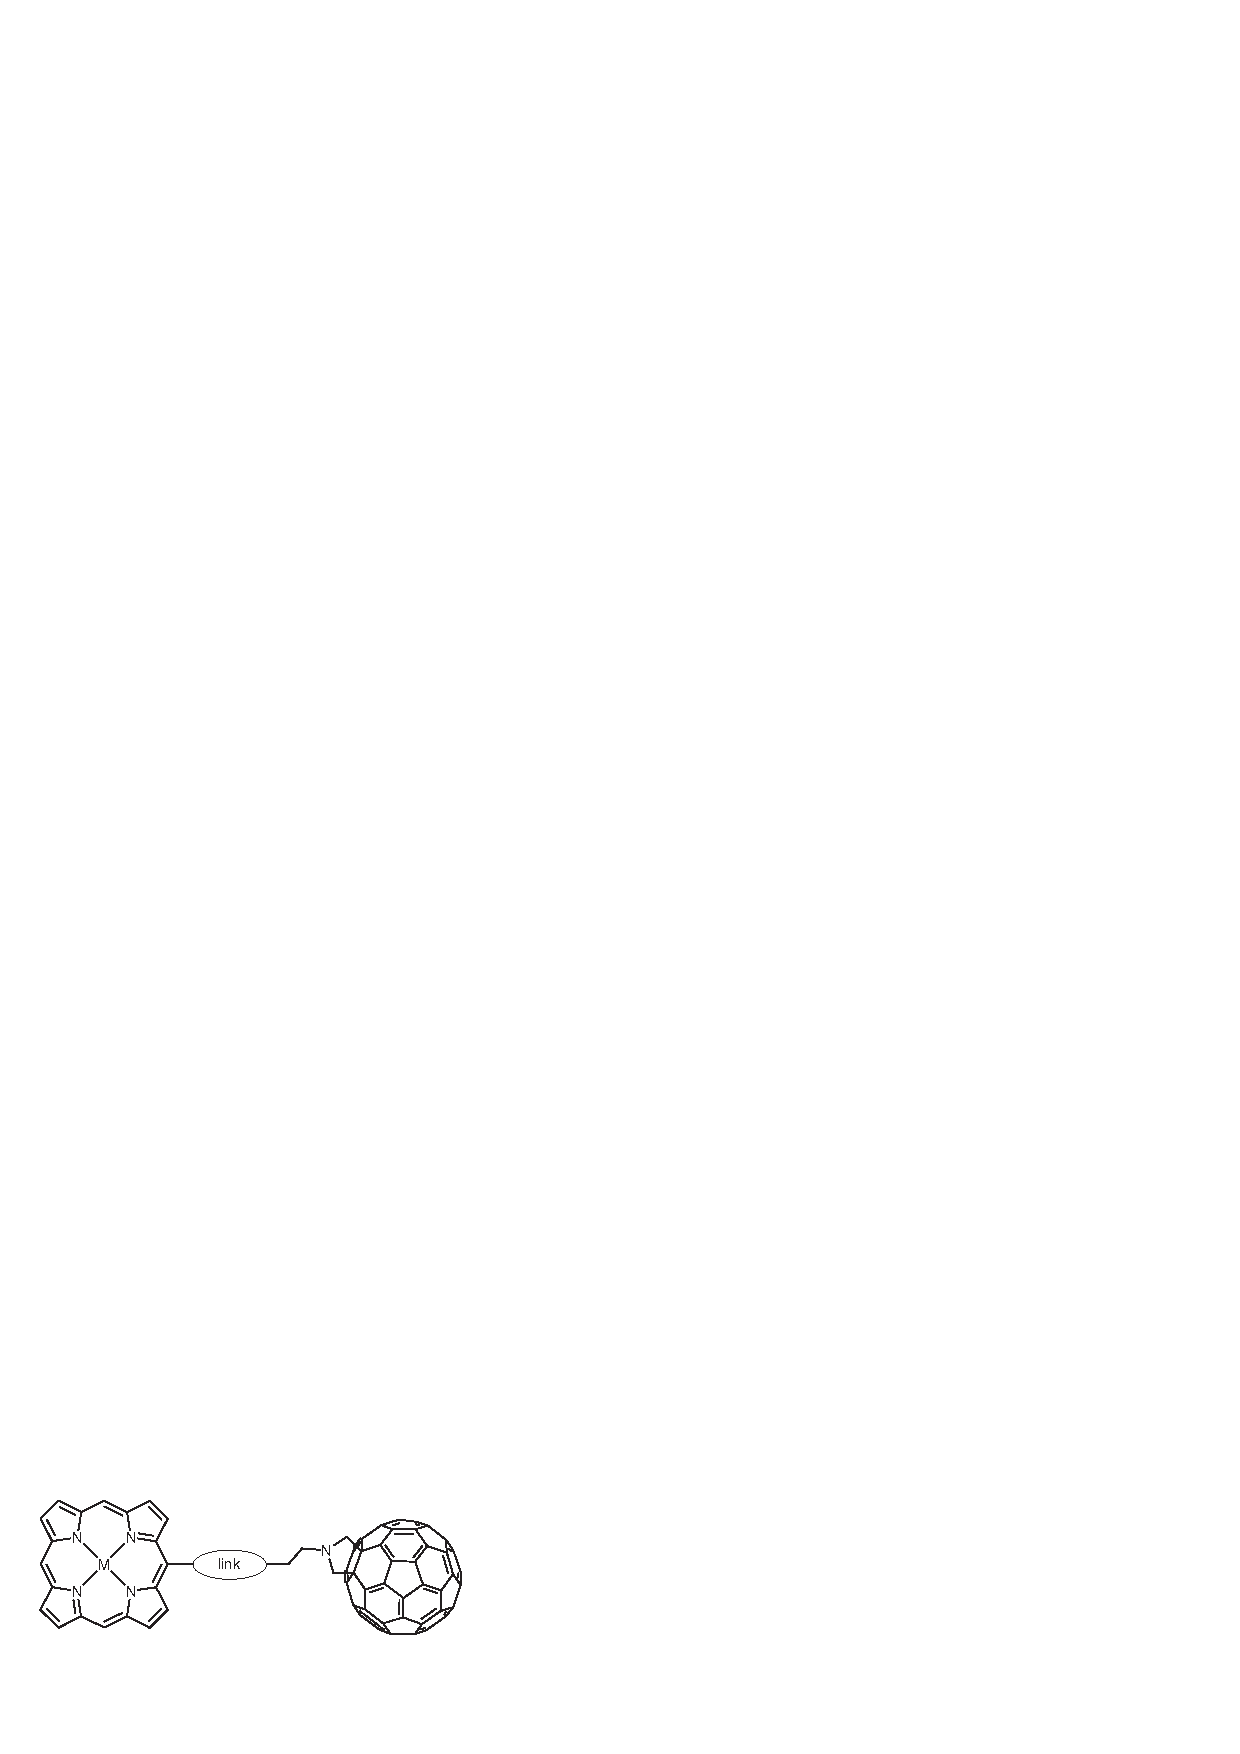
\includegraphics[valign=b]{figures/cpds/dyad.pdf} \\*
    \cmpd{dpm} & \cmpd{dyad} \\ \hline
    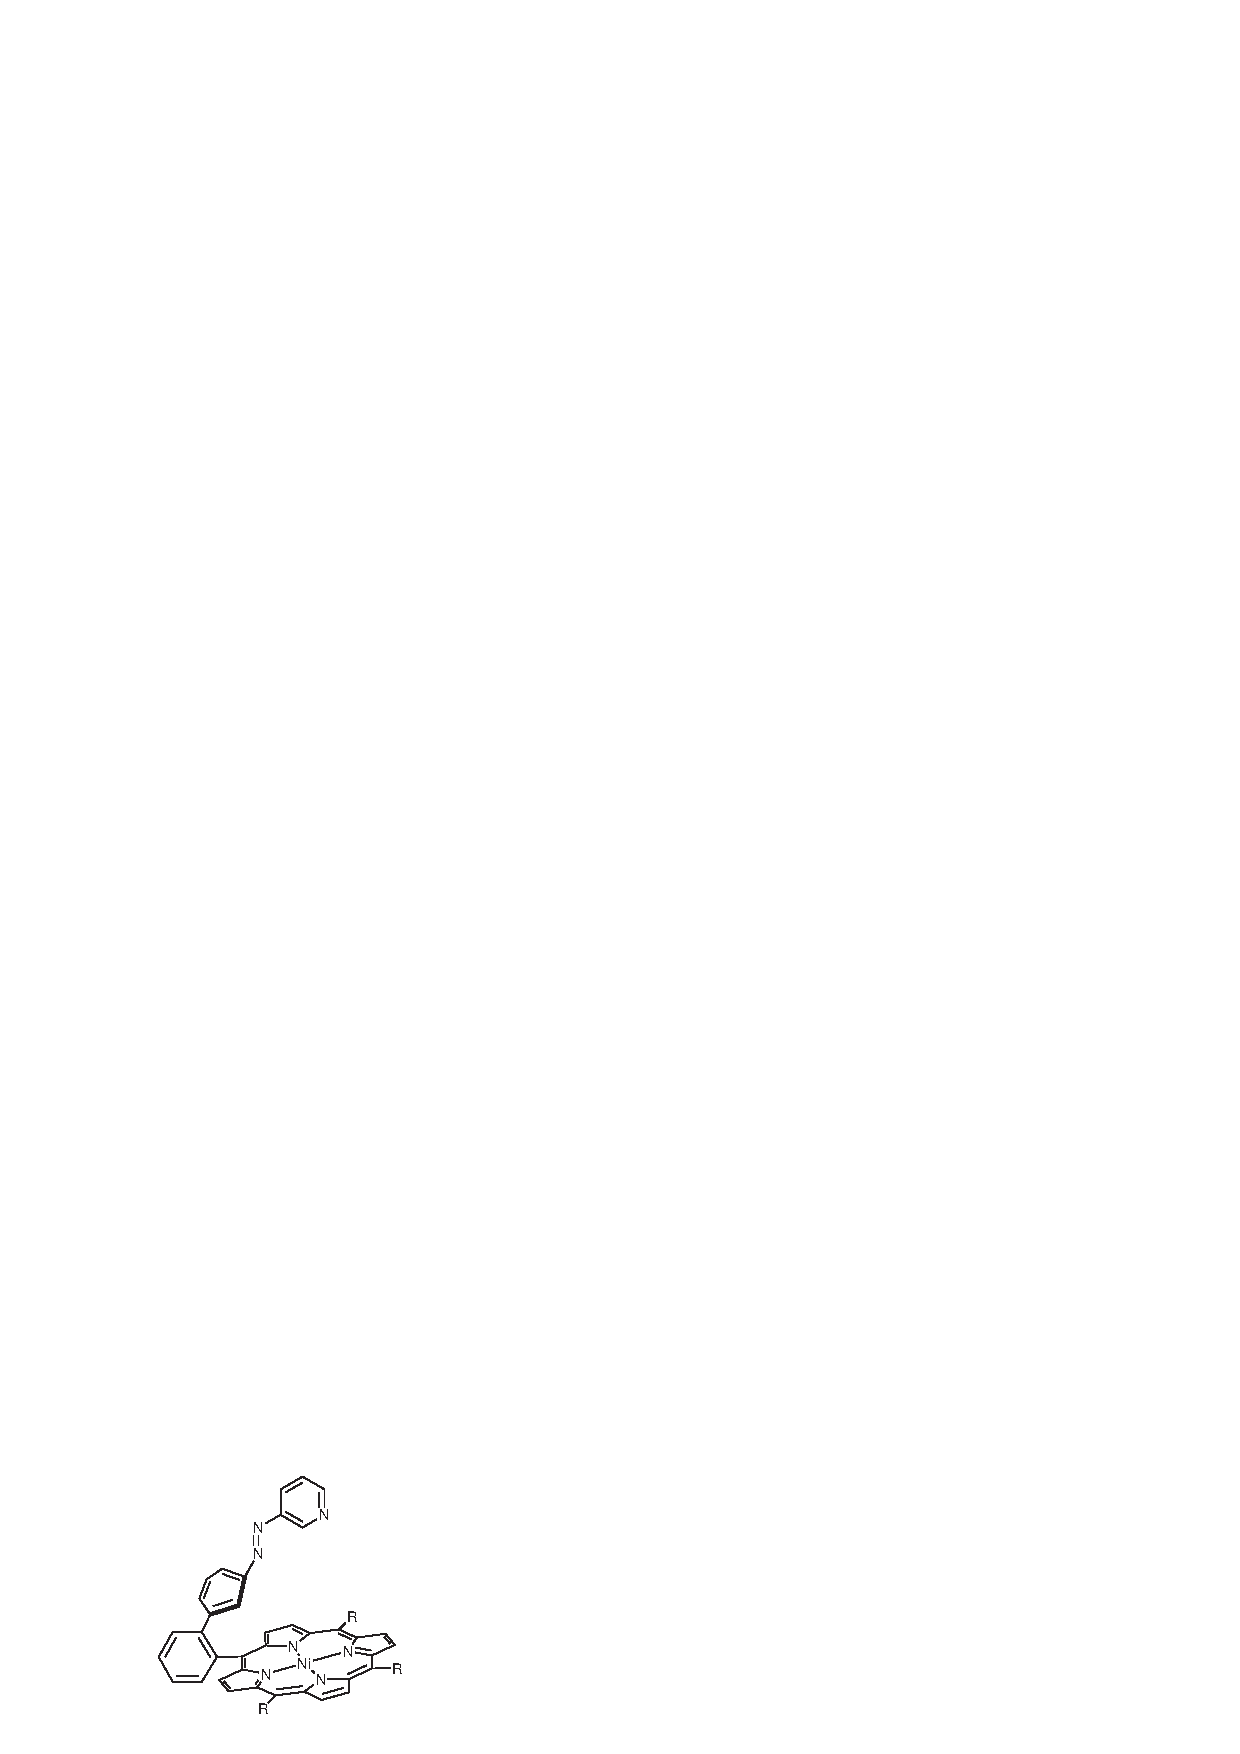
\includegraphics[valign=b]{figures/cpds/switch.pdf} & 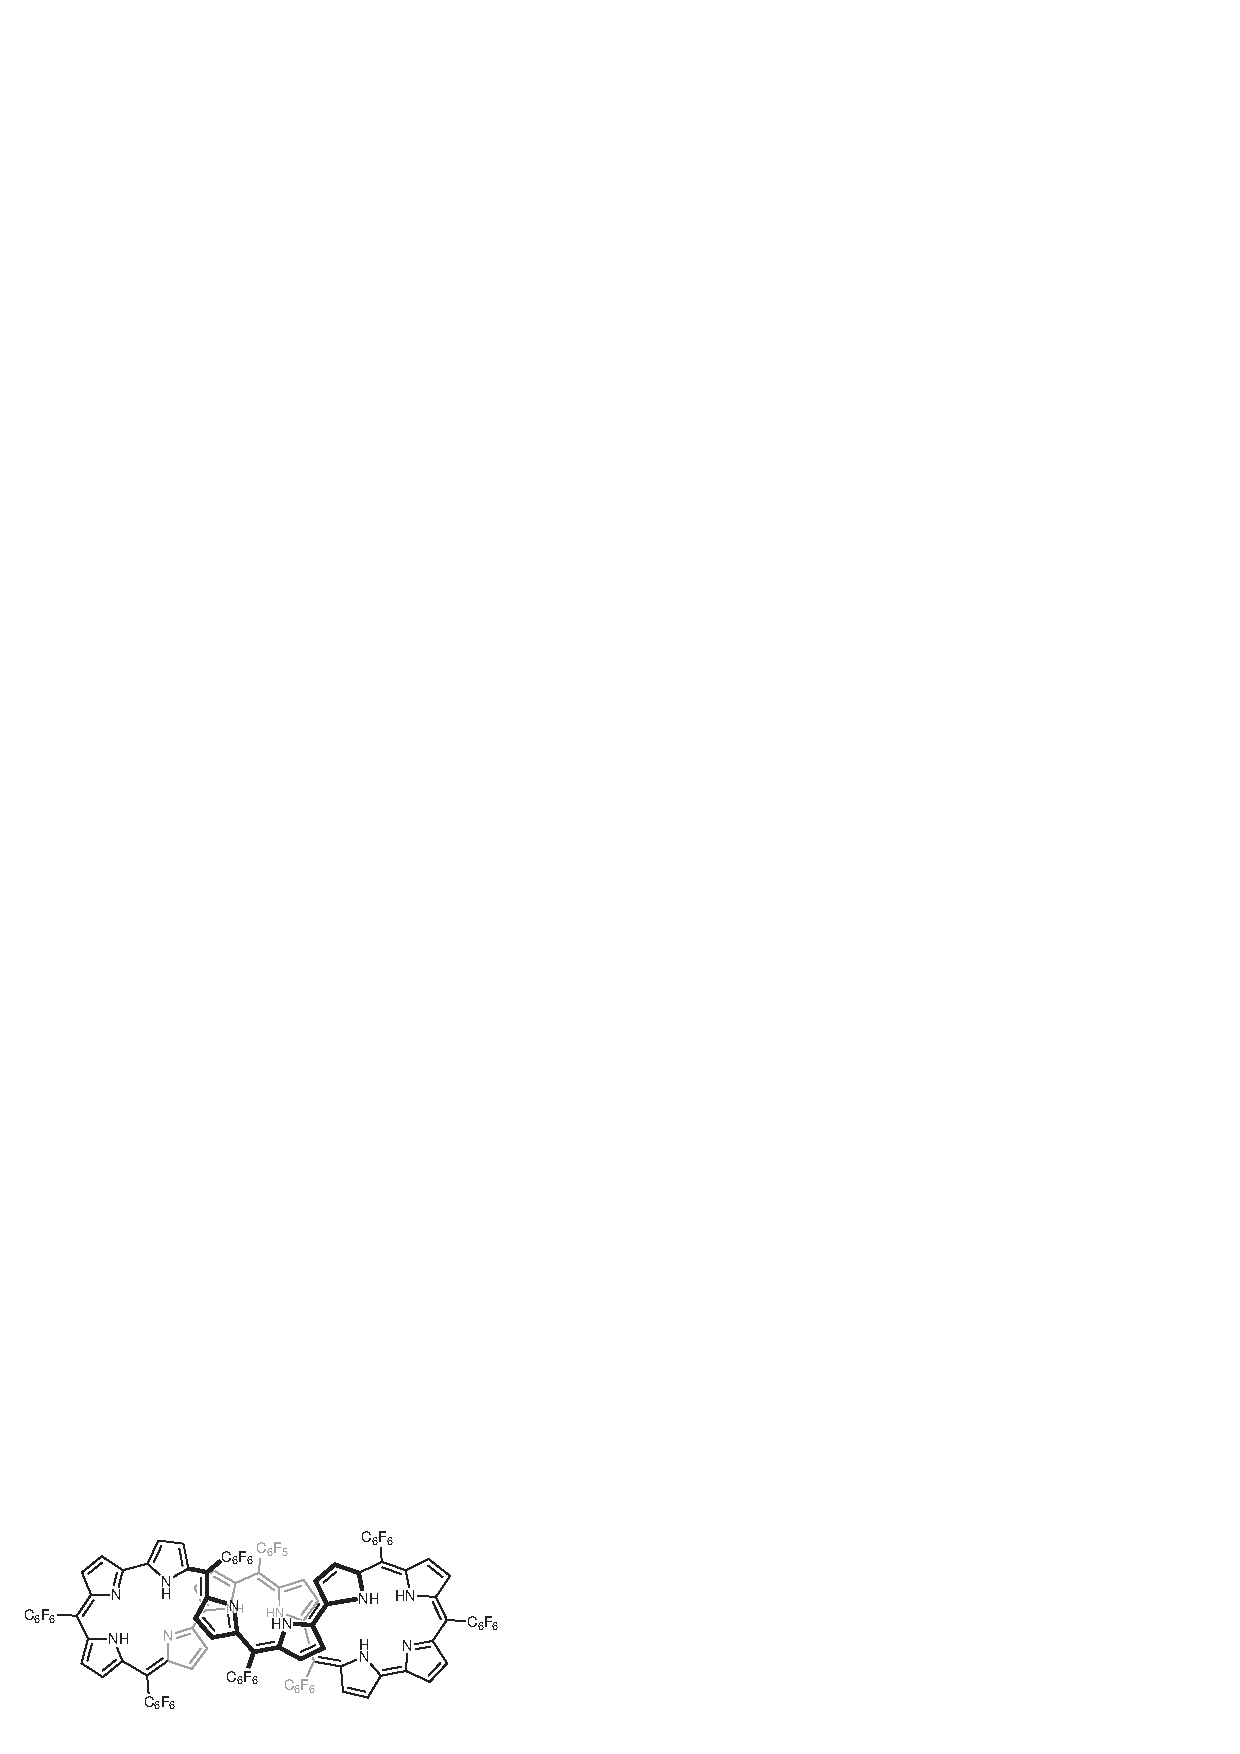
\includegraphics[valign=b]{figures/cpds/osuka52.pdf} \\*
    \cmpd{switch} & \cmpd{osuka52} \\  \hline
    \includegraphics[valign=b]{figures/cpds/benzene.pdf} & \includegraphics[valign=b]{figures/cpds/cot.pdf} \\*
    \cmpd{benzene} & \cmpd{cot} \\ \hline
    
\includegraphics[valign=b]{figures/cpds/cbd.pdf} & \includegraphics[valign=b]{figures/cpds/tenannulene.pdf} \\*
    \cmpd{cbd} & \cmpd{tenannulene} \\ \hline
    \includegraphics[valign=b]{figures/cpds/homoarom.pdf} & 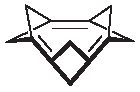
\includegraphics[valign=b]{figures/cpds/trishomoarom.pdf} \\*
    \cmpd{homoarom} & \cmpd{trishomoarom} \\  \hline
    \includegraphics[valign=b]{figures/cpds/anthracene.pdf} & 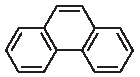
\includegraphics[valign=b]{figures/cpds/phenanthrene.pdf} \\*
    \cmpd{anthracene} & \cmpd{phenanthrene} \\ \hline
    \includegraphics[valign=b]{figures/cpds/anthYes.pdf}  & \includegraphics[valign=b]{figures/cpds/anthNo.pdf} \\*
    \cmpd{anthYes} & \cmpd{anthNo} \\ \hline
    \includegraphics[valign=b]{figures/cpds/HBC.pdf} & \includegraphics[valign=b]{figures/cpds/herges.pdf} \\*
    \cmpd{HBC} & \cmpd{herges} \\ \hline
    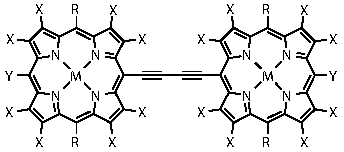
\includegraphics[valign=b]{figures/cpds/p2.pdf} & \includegraphics[valign=b]{figures/cpds/monoacfc.pdf} \\*
    \cmpd{p2} & \cmpd{monoacfc} \\ \hline





\end{longtable}
\endgroup
\end{center}
%\end{table}

%\end{multicols}